\documentclass[geometry-lectures-21.tex]{subfiles}

\begin{document}



\section{Homology and cohomology groups}\label{sec:homoology}

Next, we will learn the basics of \textbf{algebraic topology}, which studies the topology of a manifold by groups and algebras. The fundamental idea was introduced by Poincar\'e in the seminal paper \cite{poincare1895analysis} where he has conveyed the concept of homology groups and fundamental groups. His idea has been put on a mathematical rigorous footing in the early twentieth century. Let us begin with homology groups.

\subsection{Simplicial homology}

Algebraic information can be extracted from a manifold via \textbf{complexes}. Modern algebraic topology is established based on \textbf{singular complexes}. Since the technical apparatus of singular homology is somewhat complicated, we will use a more
primitive version called \textbf{simplicial homology}, which is friendly to intuitive understanding. For singular complexes, one can refer to the comprehensive textbook \cite{hatcher2005algebraic}.

The relevance is that these can be used to define simplices (which are simple, as opposed to complexes).
\bdefn[$q$-simplex]
 A \textbf{$q$-simplex} is the convex hull of $(q + 1)$ affinely independent (or general position) points $a_0, \cdots, a_q \in \bR^m$, i.e.\ the set
 \[
  \sigma = \langle a_0, \cdots, a_q\rangle = \left\{\sum_{i = 0} t_i a_i : \sum_{i = 0}^q t_i = 1,t_i \geq 0\right\}.
 \]
 The points $a_0, \cdots, a_q$ are the \textbf{vertices}, and are said to \textbf{span} $\sigma$. The $(q+1)$ tuples $(t_0, \cdots, t_q)$ are called the \textbf{barycentric coordinates} for the point $\sum t_i a_i$.



 We often denote an oriented simplex as $\sigma$, and then $\bar{\sigma}$ denotes the same simplex with the opposite orientation.
\edefn

Some examples are as follows. When $q=0$, it is a point. $q=1$, it is a line.

 \begin{minipage}[b]{2.5cm}
 \begin{center}
  \begin{tikzpicture}
   \node [circ] at (0,1) {};
    \node at (0,0) {$q=0$};
  \end{tikzpicture}
 \end{center}
   \end{minipage}
 \begin{minipage}[b]{3.5cm}
  \begin{center}
  \begin{tikzpicture}
   \node [circ] at (0, 0) {};
   \node [circ] at (2, 0) {};
   \draw (0, 0) -- (2, 0);
       \node at (1,-1) {$q=1$};
  \end{tikzpicture}
 \end{center}
   \end{minipage}
 \begin{minipage}[b]{3.5cm}
 \begin{center}
  \begin{tikzpicture}
   \draw [fill=mblue, fill opacity=0.5] (0, 0) -- (2, 0) -- (1, 1.732) -- cycle;
   \node [circ] at (0, 0) {};
   \node [circ] at (2, 0) {};
   \node [circ] at (1, 1.732) {};
          \node at (1,-.5) {$q=2$};
  \end{tikzpicture}
 \end{center}
  \end{minipage}
 \begin{minipage}[b]{3.5cm}
 \begin{center}
  \begin{tikzpicture}
   \node [circ] at (0, 0) {};
   \node [circ] at (2, 0) {};
   \node [circ] at (1, -0.5) {};
   \node [circ] at (1, 1.3) {};
   \draw [dashed] (0, 0) -- (2, 0);
   \fill [mblue, opacity=0.5] (2, 0) -- (1, -0.5) -- (1, 1.3) -- cycle;
   \fill [mblue!60!black, opacity=0.5] (0, 0) -- (1, -0.5) -- (1, 1.3) -- cycle;
   \draw (2, 0) -- (1, -0.5) -- (0, 0);
   \draw (0, 0) -- (1, 1.3) -- (2, 0);
   \draw (1, 1.3) -- (1, -0.5);
   \node at (1,-1) {$q=3$};
  \end{tikzpicture}
 \end{center}
 \end{minipage}

 A \textbf{face} of a simplex $\sigma$ is a subset (or subsimplex) spanned by a subset of the vertices. The \textbf{boundary} $\partial \sigma$ is the union of the proper faces, and the \textbf{interior} $\mathring{\sigma}$ is the complement of the boundary. We write $\tau \leq \sigma$ when $\tau$ is a face of $\sigma$. In particular, the interior of a vertex is the vertex itself. Note that this notion of interior and boundary is distinct from the topological notion of boundary.




We will now glue simplices together to build \textbf{complexes}, or \textbf{simplicial complexes} (oxymoron!).

\bdefn
 A \textbf{simplicial complex} is a finite set $K$ of simplices in $\bR^n$ such that
 \begin{enumerate}
  \item If $\sigma \in K$ and $\tau$ is a face of $\sigma$, then $\tau \in K$.
  \item If $\sigma, \tau \in K$, then $\sigma \cap \tau$ is either empty or a face of both $\sigma$ and $\tau$.
 \end{enumerate}
\edefn



\bexample
 the left is a simplicial complex, but the right is not:
 \begin{center}
  \begin{tikzpicture}
   \node [circ] at (0, 0) {};
   \node [circ] at (2, 0) {};
   \node [circ] at (3, -1) {};
   \node [circ] at (1, -0.5) {};
   \node [circ] at (1, 1.3) {};
   \node [circ] at (-1, -0.5) {};
   \draw [dashed] (0, 0) -- (2, 0);
   \fill [mblue, opacity=0.5] (2, 0) -- (1, -0.5) -- (1, 1.3) -- cycle;
   \fill [mblue!60!black, opacity=0.5] (0, 0) -- (1, -0.5) -- (1, 1.3) -- cycle;
   \draw (2, 0) -- (1, -0.5) -- (0, 0);
   \draw (0, 0) -- (1, 1.3) -- (2, 0);
   \draw (1, 1.3) -- (1, -0.5);
   \draw [fill=mblue!70!white, fill opacity=0.5] (2, 0) -- (3, -1) -- (1, -0.5);

   \draw (0, 0) -- (-1, -0.5);
   \draw [fill=mblue, fill opacity=0.5] (-3, -0.5) -- (-1, -0.5) -- (-2, -1.2) -- cycle;
   \node [circ] at (-3, -0.5) {};
   \node [circ] at (-1, -0.5) {};
   \node [circ] at (-2, -1.2) {};

   \draw (-1.5, -0.2) node [circ] {} -- (-1.2, 1) node [circ] {};
 \end{tikzpicture}\hspace{2cm}
    \begin{tikzpicture}
      \node [circ] at (2,0){};
      \node [circ] at (3,-0.5){};
        \node [circ] at (3,1){};
        \node [circ] at (3,0){};
        \node [circ] at (5,0.3){};
            \draw[fill,mblue, opacity=0.5] (2, 0) -- (3, -0.5) -- (5,0.3) -- (3, 1)--cycle;
      \draw (2, 0) -- (3, -0.5) -- (5,0.3) -- (3, 1)--cycle;
      \draw (3, -0.5) -- (3, 1);
      \draw (2,0) -- (3,0);
        \end{tikzpicture}
 \end{center}
\eexample
Technically, a simplicial complex is defined to be a set of simplices, which is just collections of points. It is not a subspace of $\bR^n$. The \textbf{polyhedron} defined by $K$ is the union of the simplices in $K$, and denoted by $|K|$. The \textbf{dimension} of $K$ is the highest dimension of a simplex of $K$. The \textbf{$d$-skeleton} $K^{(d)}$ of $K$ is the union of the $n$-simplices in $K$ for $n \leq d$.
 A \textbf{triangulation} of a space $M$ is a homeomorphism $h: |K| \to M$, where $K$ is some simplicial complex.


\bexample
 Let $\sigma$ be the standard $(n+1)$-simplex. The boundary $\partial \sigma$ is homeomorphic to $S^{n}$ (e.g.\ the boundary of a (solid) triangle is the boundary of the triangle, which is also a circle) . This is called the \textbf{simplicial $n$-sphere}.
\eexample

We can also triangulate our $S^n$ in a different way:
\bexample
 In $\bR^{n + 1}$, consider the simplices $ \langle \pm \mathbf{e}_0, \cdots, \pm \mathbf{e}_n\rangle$ for each possible combination of signs. So we have $2^{n + 1}$ simplices in total. Then their union defines a simplicial complex $K$, and
 \[
  |K| \cong S^n.
 \]
 \begin{center}
  \begin{tikzpicture}
   \draw [gray, ->] (-2, 0) -- (2, 0);
   \draw [gray, ->] (0, -2) -- (0, 2);
   \draw [gray, ->] (0.894, 1.788) -- (-0.894, -1.788);

   \node [circ] (x1) at (1, 0) {};
   \node [circ] (x2) at (-1, 0) {};
   \node [circ] (z1) at (0, 1) {};
   \node [circ] (z2) at (0, -1) {};
   \node [circ] (y1) at (-0.3, -0.6) {};
   \node [circ] (y2) at (0.3, 0.6) {};

   \draw (x1) -- (y1) -- (z1) -- (x1) -- (z2) -- (y1) -- (x2) -- (z1);
   \draw (z2) -- (x2);
   \draw [dashed] (x2) -- (y2) -- (x1);
   \draw [dashed] (z2) -- (y2) -- (z1);
  \end{tikzpicture}
 \end{center}
\eexample
The nice thing about this triangulation is that the simplicial complex is invariant under the antipodal map. So not only can we think of this as a triangulation of the sphere, but a triangulation of $\RP^n$ as well.





  An \textbf{oriented $q$-simplex} in a simplicial complex $K$ is $\langle a_0, \cdots, a_q\rangle \in K$ with ordering of vertices where two $(q + 1)$-simplices $\langle a_0, \cdots, a_q\rangle$ and $\langle a_{\pi(0)}, \cdots, a_{\pi(q)}\rangle$ are the same \textbf{oriented} simplex if $\pi \in \mathfrak{S}_{q+1}$ is an \textbf{even} permutation.



\bdefn[Chain group $C_q(K)$]\label{def:chain}
 Let $K$ be a simplicial complex and let $\{\sigma_1, \cdots, \sigma_\ell\}$ span $K^{(q)}$ with orientation. Then we define $C_q(K)$ be the free abelian group (free $\bZ$-module) with basis $\{\sigma_1, \cdots, \sigma_\ell\}$, i.e.\ $$C_q(K) \cong \bZ \sigma_1\oplus\cdots \oplus\bZ\sigma_\ell~.$$
\edefn

(See Definition \ref{def:module} for a $\bZ$-module.)
 We define \textbf{boundary homomorphisms}
 \[
  \partial_q: C_q(K) \to C_{q- 1}(K);~
  \langle a_0, \cdots, a_q\rangle \mapsto \sum_{i = 0}^q (-1)^i \langle a_0, \cdots, \widehat{a}_i, \cdots, a_q\rangle~,
 \]
 where $\langle a_0, \cdots, \widehat{a}_i, \cdots, a_q\rangle = \langle a_0, \cdots, a_{i - 1}, a_{i + 1}, a_q\rangle$ is the simplex with $a_i$ removed. We can show that $\partial_{q-1}\cdot \partial_q=0$. Hence, given a complex $K$, one obtains a chain complex $(C_{\bullet}(K),\partial)$.




\bdefn[Chain complex]
 A \textbf{chain complex} $(C_{\bullet},\partial)$ is a sequence of chain groups $C_0, C_1, C_2, \cdots$ equipped with boundary maps $\partial_q: C_q \to C_{q- 1}$ such that $\partial_{q- 1} \circ \partial_q = 0$ for all $q$:
 \[
  0\xrightarrow{\partial_{n+1}}C_n\xrightarrow{\partial_{n}}C_{n-1}\xrightarrow{\partial_{n-1}}\cdots \xrightarrow{\partial_{2}} C_1\xrightarrow{\partial_{1}}C_0\xrightarrow{\partial_{0}}0
 \]
\edefn

Notice that it is very similar to de Rham complex \eqref{deRham-complex}, but degrees of complexes are decreasing by $\partial$ here.
As in the de Rham cohomology \eqref{deRham-cohomology}, we define the \textbf{$q$-cycles} and the \textbf{$q$-boundaries} of the chain complex $C_\bullet(K)$ of a complex $K$
 \[
  Z_q(K) = \Ker \partial_q~,\quad
  B_q(K) = \Im \partial_{q+1}~.
 \]
 Then, the \textbf{$q$-th homology group} of $C_{\bullet}$ is defined to be
 \[
  H_q(K;\bZ) = \frac{\Ker \partial_q}{\Im \partial_{q+ 1}} = \frac{Z_q(K)}{B_q(K)}.
 \]

Given a triangulated manifold $|K|\to M$, it is obvious that a chain complex depends on a complex $K$. However, as we will see briefly below, the homology group is independent of a triangulation of $M$. Namely, for two triangulation $|K|\to M$, $|K'|\to M$, we have
$$ H_q(K;\bZ)\cong H_q(K';\bZ)~,$$
so that we can write it as $H_q(M;\bZ)$. As we will see below, homology groups are homotopy-invariant, and therefore \textbf{topological invariant}. It is a $\bZ$-module so that it may contain a torsion subgroup like $\bZ_m$ according to Theorem \ref{thm:module}.

In Definition \ref{def:chain}, one can consider a free $\bR$-module $C_q(K;\bR)$ instead of $\bZ$-module. Then, the corresponding homology group is denoted by $H_q(K;\bR)$. Given a triangulation $h: |K| \to M$ of a manifold $M$, the dimension of $H_q(K;\bR)$ is called the $q$-th \textbf{Betti number}.
 The \textbf{Euler characteristic} of a triangulated space $h: |K| \to M$ is the alternative sum of dimensions of real-valued homology groups
 \[
  \chi(M) = \sum_{i \geq 0} (-1)^i \dim H_i(M; \bR).
 \]


Let $|K|\to M$ be a triangulation of an $n$-dimensional oriented closed connected manifold $M$. Then, the $n$-th homology group is $H_n(K,\bZ)\cong \bZ$ and its generator is denoted by $[M]$ and called the \textbf{fundamental class}.



\bexample\label{ex:S1}
 Let $K$ be the standard simplicial $1$-sphere, ie, we have the following in $\bR^3$.
 \begin{center}
  \begin{tikzpicture}
   \draw [->] (0, 0) -- (3, 0);
   \draw [->] (0, 0) -- (0, 3);
   \draw [->] (0, 0) -- (-1, -2);

   \draw [->-=0.58] (2, 0) -- (0, 2);
   \draw [->-=0.58] (0, 2) -- (-0.5, -1);
   \draw [->-=0.58] (-0.5, -1) -- (2, 0);

   \node [left] at (-0.5, -1) {$a_0$};
   \node [below] at (2, 0) {$a_1$};
   \node [right] at (0, 2) {$a_2$};

   \node [circ] at (-0.5, -1) {};
   \node [circ] at (2, 0) {};
   \node [circ] at (0, 2) {};
  \end{tikzpicture}
 \end{center}
 Our simplices are thus
 \[
  K = \{\langle a_0\rangle, \langle a_1\rangle, \langle a_2\rangle, \langle a_0, a_1\rangle, \langle a_1, a_2\rangle, \langle a_2, a_0\rangle\}.
 \]
 Our chain groups are
 \begin{align*}
   C_0\langle K\rangle &= \{ \langle a_0\rangle , \langle a_1\rangle , \langle a_2\rangle \} \cong \bZ^3\\
   C_1\langle K\rangle &= \{ \langle a_0, a_1\rangle , \langle a_1, a_2\rangle , \langle a_2, a_0\rangle  \} \cong \bZ^3.
 \end{align*}
 All other chain groups are zero.

 Hence, the only non-zero boundary map is
 \[
  \partial_1: C_1(K) \to C_0(K).
 \]
 We can write down its matrix with respect to the given basis.
 \[
  \begin{pmatrix}
   -1 & 0 & 1\\
   1 & -1 & 0\\
   0 & 1 & -1
  \end{pmatrix}
 \]
 We now have everything we need to know about the homology groups, and we just need to do some linear algebra to figure out the image and kernel, and thus the homology groups. We have
 \[
  H_0(K;\bZ) = \frac{\Ker (\partial_0: C_0(K) \to C_{-1}(K))}{\Im (\partial_1: C_1(K) \to C_0(K))} \cong \frac{C_0(K)}{\Im \partial_1} \cong \frac{\bZ^3}{\Im \partial_1}.
 \]
 After doing some row operations with our matrix, we see that the image of $\partial_1$ is a two-dimensional subspace generated by the image of two of the edges. Hence we have
 \[
  H_0(K;\bZ) = \bZ.
 \]
 We interpret this to mean $K$ has one path-connected component. In fact, generators of $H_0(K;\bZ)$ represent path-connected components of $K$. If $K$ has $r$ path-connected components, then we expect $H_0(K;\bZ)\cong \bZ^r$.

 Similarly, we have
 \[
  H_1(K;\bZ) = \frac{\Ker \partial_1}{\Im \partial_2} \cong \Ker \partial_1.
 \]
 It is easy to see that we have
 \[
  \Ker \partial_1 = \bZ\{ \langle a_0, a_1\rangle + \langle a_1, a_2\rangle + \langle a_2, a_0\rangle\} \cong \bZ.
 \]
 So we also have
 \[
  H_1(K;\bZ) \cong \bZ.
 \]
 We see that this $H_1(K;\bZ)$ is generated by precisely the single loop in the triangle, which is the fundamental class $[S^1]$. The fact that $H_1(K;\bZ)$ is non-trivial means that we do indeed have a hole in the middle of the circle.
\eexample

We can also consider a map between two simplicial complexes.

\bdefn[Simplicial map]
 A \textbf{simplicial map} $f: K \to K'$ is a function $f: V_K \to V_{K'}$ such that if $\langle a_0, \cdots, a_q\rangle$ is a simplex in $K$, then $\{f(a_0), \cdots, f(a_q)\}$ spans a simplex of $K'$.
\edefn

\bexample
 the left is a simplicial map, but the right is not:

  \begin{tikzpicture}[scale=.8]
    \draw[fill,mblue, opacity=0.5] (2, 0)-- (3, -0.5) -- (3, 1) --cycle;
\draw (2, 0) node[black,left] {$a_1$}-- (3, -0.5) node[black,below] {$a_2$} -- (3, 1) node[black,above] {$a_3$} --cycle;
\draw (3,-0.5) -- (4,.5) node[right]{$a_4$};
\draw[->] (5,0) to node[below]{$f$} (6,0);
\draw (7,1) node[above]{$f(a_1)=f(a_3)$} -- (7.25,-.5) node[below]{$f(a_2)$} -- (8,.5) node[right]{$f(a_4)$};
\node [circ] at (2,0) {};
\node [circ] at (3,-0.5){};
\node [circ] at (3,1){};
\node [circ] at (3,-0.5){};
\node [circ] at (4,.5){};
\node [circ] at (7,1){};
\node [circ] at (7.25,-.5){};
\node [circ] at (8,.5){};
\end{tikzpicture}\hspace{1cm}
 \begin{tikzpicture}[scale=.8]
   \draw[fill,mblue, opacity=0.5] (2, 0)-- (3, -0.5) -- (3, 1) --cycle;
\draw (2, 0) node[black,left] {$a_1$}-- (3, -0.5) node[black,below] {$a_2$} -- (3, 1) node[black,above] {$a_3$} --cycle;
\draw (3,-0.5) -- (4,.5) node[right]{$a_4$};
\draw[->] (5,0) to node[below]{$f$} (6,0);
\draw (7,1) node[above]{$f(a_1)$} -- (7.25,-.5) node[below]{$f(a_2)$} -- (8,.5) node[right]{$f(a_3)=f(a_4)$};
\node [circ] at (2,0){};
\node [circ] at (3,-0.5){};
\node [circ] at (3,1){};
\node [circ] at (3,-0.5){};
\node [circ] at (4,.5){};
\node [circ] at (7,1){};
\node [circ] at (7.25,-.5){};
\node [circ] at (8,.5){};
\end{tikzpicture}

\eexample



A simplicial map $f$ induces a homomorphism among chain groups
$$
f_*:C_\bullet(K)\to C_\bullet(K')
$$
by
$$
f_*(\langle a_0,a_1,\ldots,a_q\rangle)=\begin{cases} \langle f(a_0), f(a_1),\ldots,f(a_q)\rangle&\textrm{if} \ f(a_i)\neq f(a_j) \ \textrm{for all}\ i \neq j \\ 0 & \textrm{if} \ f(a_i)=f(a_j) \ \textrm{for some}\ i \neq j \end{cases}~.
$$
for a $q$-simplex $\sigma=\langle a_0,a_1,\ldots,a_q\rangle\in C_q(K)$.
This induced homomorphism satisfies
$$
\partial \cdot f_*=f_*\cdot \partial~
$$
Therefore, we have the chain map
\bdefn[Chain map]
 A chain map $f_{\bullet}: C_{\bullet}(K) \to C_{\bullet}(K')$ is a sequence of homomorphisms $f_q:C_{q}(K) \to C_{q}(K')$ such that
 \[
  f_{q-1} \circ \partial_q = \partial_q \circ f_q
 \]
 for all $n$. In other words, the following diagram commutes:
 \[
  \begin{tikzcd}[row sep=large]
 \cdots \ar [r, "\partial_{q+1}"] &  C_q(K) \ar [r, "\partial_q"] \ar[d, "f_q"] & C_{q-1}(K) \ar[d, "f_0"]\ar [r, "\partial_{q-1}"]& \cdots \ar [r, "\partial_2"] &  C_1(K) \ar [r, "\partial_1"] \ar[d, "f_1"] & C_0(K) \ar[r, "\partial_0"] \ar[d, "f_{q-1}"] &  0  \\ \cdots \ar [r, "\partial_{q+1}"]
 &  C_q(K') \ar [r, "\partial_q"] & C_{q-1}(K')  \ar [r, "\partial_{q-1}"]& \cdots \ar [r, "\partial_2"] &  C_1(K') \ar [r, "\partial_1"] & C_0(K') \ar[r, "\partial_0"] &  0
  \end{tikzcd}
 \]
\edefn

 Hence it also induces $f_*: H_n(K;\bZ) \to H_n(K';\bZ);[z] \mapsto [f(z)]$. The following theorem is very important for homotopy-invariance of homology groups. Using this theorem, it is easy to prove that the homology group of a topological space $M$ is independent of the choice of triangulations.


\bthm\label{thm:inducedeq}
Let $K, K^{\prime}$ be simplicial complexes and $F:K\times I\to K'$ be a simplicial map. If we denote the restricted maps as $f_0=F|_{K\times\{0\}}$ and $f_1=F|_{K\times\{1\}}$, then the two induced homomorphisms of homology groups are identical
$$
f_{0*}=f_{1*} : H_{*}(K;\bZ) \rightarrow H_{*}(K^{\prime};\bZ)~.
$$
\ethm
Since this is an important theorem, we give a sketch of a proof.
Let us denote vertices $a_i\times \{0\}$ and $a_i\times \{1\}$ of a simplicial complex $K\times I$ by $\underline a_i$ and $\overline a_i$. Let us define a homomorphism $D:C_q(K)\to C_{q+1}(K\times I)$ by
$$\langle a_0,a_1,\ldots,a_q\rangle \mapsto \sum_{i=0}^{q}(-1)^{i} \left\langle\underline{a}_{0}, \underline{a}_{1}, \ldots, \underline{a}_{i}, \overline{a}_{i}, \dots, \overline{a}_{q}\right\rangle~.$$
Then, one can show that
$$(\partial_{q+1} D_{q}+D_{q-1} \partial_{q})\left(\langle a_{0}, a_{1}, \cdots, a_{q}\rangle\right) =\langle\overline{a}_{0}, \overline{a}_{1}, \cdots, \overline{a}_{q}\rangle-\langle\underline{a}_{0}, \underline{a}_{1}, \cdots, \underline{a}_{q}\rangle~.$$
If we denote the elements corresponding to $z\in Z_q(K)$ by $\underline{z} \in Z_{q}(K\times \{0\})$ and $\overline{z} \in Z_{q}(K\times \{1\})$, then we have
$$
\left(\partial_{q+1} D_{q}+D_{q-1} \partial_{q}\right)(z)=\overline{z}-\underline{z}~.
$$
Therefore, the difference of $(f_0)_*$ and $(f_1)_*$ is exact
$$
F(\partial_{q+1} D_{q})(z)=(f_1)_*(z)-(f_0)_*(z)~.
$$
Hence, $(f_0)_*=(f_1)_*$.





\subsection{Mayer-Vietoris exact sequence}\label{sec:Mayer-Vietoris}

We just briefly explain a powerful theorem called Mayer-Vietoris sequence to compute homology. For more detail, I refer to \cite[p.149]{hatcher2005algebraic}. A sequence of homomorphisms $\{f_q\}$ between modules $M_q$
$$
\cdots \xrightarrow{f_{q+2}} M_{q+1}\xrightarrow{f_{q+1}} M_{q}\xrightarrow{f_{q}} M_{q-1}\xrightarrow{f_{q-1}} \cdots
$$
is called an \textbf{exact sequence} if $$\Im f_{q+1}=\Ker f_q \qquad \textrm{for} \ \ \forall q~.$$
Notice the difference from a Chain complex where $\Im \partial_{q+1}\in\Ker \partial_q$, so that a Chain complex is \textbf{not} an exact sequence.

Let $K$ be a simplicial complex, and $K_1,K_2$ are subcomplexes such that $K = K_1\cup K_2$. Moreover, $K'=K_1 \cap K_2$ is also a subcomplex of $K$.
\begin{center}
 \begin{tikzpicture}
  \draw [fill=mred, fill opacity=0.3] (-1, 0) ellipse (1.5 and 0.6);
  \draw [fill=mblue, fill opacity=0.3] (1, 0) ellipse (1.5 and 0.6);
  \node at (-2.2, 0) {$K_1$};
  \node at (2.2, 0) {$K_1$};
    \node at (0, 0) {$K'$};
 \end{tikzpicture}
\end{center}
Then, we have the following inclusion maps:
\[
 \begin{tikzcd}
  K' \ar[r, hook, "i"] \ar[d, hook, "j"] & K_1\ar[d, hook, "k"]\\
  K_2 \ar[r, hook, "\ell"] & K.
 \end{tikzcd}
\]
Then, for $
[z^{\prime}] \in H_{q}(K^{\prime}),\ [z_{1}] \in H_{q}(K_{1}),\ [z_{2}] \in H_{q}(K_{2})$, we define homomorphisms
$$
\begin{aligned} \varphi & : H_{q}(K^{\prime}) \rightarrow H_{d}(K_{1}) \oplus H_{q}(K_{2});~[x']\mapsto (i_*[x'],-j_*[x']) \\ \psi & : H_{q}(K_{1}) \oplus H_{q}(K_{2}) \rightarrow H_{q}(K);~ ([x_1], [x_2])\mapsto k_*[x_1]+\ell_*[x_2]~.\end{aligned}
$$
Furthermore, for $[z] \in H_{q}(K)$, we decompose it as
$$
z=c_{1}+c_{2}\qquad(c_{1} \in C_{q}(K_{1}), c_{2} \in C_{q}(K_{2}))~.
$$
Then, we define
$$
\Delta : H_{q}(K) \rightarrow H_{q-1}(K^{\prime}); ~ [z]\mapsto [\partial c_1]=-[\partial c_2]~.
$$
One can show that this map is independent of the choice of a representative of $[z]$, and the way of the decomposition $z=c_1+c_2$.
The theorem tells us how to compute the homology of the union $K=K_1\cup K_2$ in terms of those of $K_1,K_2$ and $K'$.


\bthm[Mayer-Vietoris]
The following sequence obtained from $\varphi, \psi, \Delta$ is a \textbf{exact sequence}:
$$
\begin{array}{cccccccc}\cdots &\xrightarrow{\Delta}& H_{q+1}(K') &\xrightarrow{\varphi}& H_{q+1}(K_1) \oplus H_{q+1}(K_2) &\xrightarrow{\psi}&H_{q+1}(K)&\\
   &\xrightarrow{\Delta}& H_{q}(K') &\xrightarrow{\varphi}&H_{q}(K_1) \oplus H_{q}(K_2) &\xrightarrow{\psi}& H_{q}(K)&\rightarrow \cdots
   \\ \cdots &\xrightarrow{\Delta}&H_{1}(K') &\xrightarrow{\varphi}&H_{1}(K_1) \oplus H_{1}(K_2) &\xrightarrow{\psi}&H_{1}(K)&\\
   &\xrightarrow{\Delta}&H_{0}(K') &\xrightarrow{\varphi}&H_{0}(K_1) \oplus H_{0}(K_2) &\xrightarrow{\psi}& H_{0}(K) &\rightarrow 0\end{array}
  $$
\ethm


\bexample
Let us compute the homology group of $n$-sphere by the Mayer-Vietoris sequence. We have obtained the homology group of $S^1$ in Example \ref{ex:S1}, and we will compute it by an induction on $n$. Suppose that the homology group of $S^{n-1}$ is
$$H_{q}(S^{n-1})=\begin{cases}\mathbb{Z} & q=0,n-1\\ 0 &\textrm{otherwise}\end{cases}~.$$
We decompose an $n$-sphere into the northern and southern hemisphere
$$\begin{aligned} K_1 &=\left\{(x^{1}, x^{2}, \cdots, x^{n+1}) \in S^{n} | x^{n+1} \geq 0\right\} \\ K_2 &=\left\{(x^{1}, x^{2}, \cdots, x^{n+1}) \in S^{n} | x^{n+1} \leqq 0\right\} \end{aligned}$$
Then, the Poincare lemma \eqref{thm:Poincare2} is
$$H_{q}(K_1)=H_{q}(K_2)=\left\{\begin{array}{ll}{\mathbb{Z}} & {(q=0} \\ {0} & {(q \neq 0}\end{array}\right.$$
By the assumption of the induction, we have
$$H_{q}(K')=H_{q}(S^{n-1})=\left\{\begin{array}{l}{\mathbb{Z}} \\ {0}\end{array}\right.$$
Then, the Mayer-Vietoris exact sequence leads to
$$
0 \rightarrow H_{q}(S^{n}) \rightarrow H_{q-1}(S^{n-1}) \rightarrow 0
$$
for $q\ge2$. For the $q=0$ degree, $\varphi$ is an injection so that $H_1(S^n;\bZ)=0$. In addition, $\psi$ is surjective so that $H_0(S^n;\bZ)=\bZ$. Therefore, we obtain
$$H_{q}(S^{n})=\begin{cases}\mathbb{Z} & q=0,n\\ 0 &\textrm{otherwise}\end{cases}~.$$
\eexample




\subsection{Homotopy invariance of homology groups}



In topology, we study spaces up to ``continuous deformation''. Famously, a coffee mug can be continuously deformed into a doughnut, and thus they are considered to be topologically the same. Now we also talk about maps between topological spaces. So a natural question is if it makes sense to talk about the continuous deformations of maps. It turns out we can, and the definition is sort-of the obvious one:

\begin{figure}[ht]\centering
\includegraphics{pictures/homotopy}
\end{figure}


\bdefn[Homotopy]\index{homotopy}
 Let $M, N$ be a topological space. A \textbf{homotopy} between $f_0, f_1: M\to N$ is a map $F: [0, 1] \times M\to N$ such that $F(0, x) = f_0(x)$ and $F(1, x) = f_1(x)$. If such an $F$ exists, we say $f_0$ is \textbf{homotopic} to $f_1$, and write $f_0 \simeq f_1$.
\edefn



\begin{figure}[ht]\centering
\includegraphics{pictures/equiv-homotopy}
\end{figure}

As easily can be seen from the figure above, homotopy $\simeq$ defines an equivalence relation on the set of maps from $M$ to $N$.
In algebraic topology, we study quantities invariant under homotopy.


\bdefn[Homotopy equivalence]\index{homotopy equivalence}
 A map $f: M\to N$ is a \textbf{homotopy equivalence} if there is some $g: N\to M$ such that $f \circ g \simeq \id_M$ and $g \circ f \simeq \id_N$. We call $g$ the \textbf{homotopy inverse}\index{homotopy inverse} to $f$.
\edefn


 If $f_0 \simeq f_1: M\to N$ and $g_0 \simeq g_1: N \to L$, then $g_0 \circ f_0 \simeq g_1 \circ f_1:M \to L$.
 \[
  \begin{tikzcd}
   M \ar[r, bend left, "f_0"] \ar[r, bend right, "f_1"'] & N \ar[r, bend left, "g_0"] \ar[r, bend right, "g_1"'] & L
  \end{tikzcd}
 \]
Therefore, homotopy equivalence is an equivalence relation.

%\bexample[Stupid example]
% If $f: M\to N$ is a homeomorphism, then it is a homotopy equivalence --- we take the actual inverse for the homotopy inverse since equal functions are homotopic.
%\eexample

A \textbf{deformation retraction} of a space $M$ onto a subspace $N\subset M$ is a family of maps $f_{t}:M \rightarrow M$, $t \in I$, such that $f_{0}=\textrm{id}$, $f_{1}(X)=A$, and $f_{t} \mid A=\textrm{id}$ for all $t$. A deformation retraction $f_{t}: X \rightarrow X$ is a special case of a homotopy.

\bexample
 Let $i: \{0\} \to \bR^n$ be the inclusion map. A homotopy equivalence can be constructed by
 $F: [0, 1] \to \bR^n \to \bR^n$ be
 \[
  F(t, \mathbf{v}) = t\mathbf{v}.
 \]
 We have $F(0, \mathbf{v}) = 0$ and $F(1, \mathbf{v}) = \mathbf{v}$. From the point of view of homotopy, the point $\{0\}$ is equivalent to $\bR^n$, so that dimension is irrelevant.
\eexample


\bexample
 Let $S^n \subseteq \bR^{n + 1}$ be the unit sphere, and $i: S^n \hookrightarrow \bR^{n + 1} \setminus \{0\}$. We show that this is a homotopy equivalence. We define $r: \bR^{n + 1} \setminus \{0\} \to S^n$ by
 \[
  r(\mathbf{v}) = \frac{\mathbf{v}}{\|\mathbf{v}\|}.
 \]
It is easy to see $r \circ i = \id_{S^n}$. In the other direction, we need to construct a path from each $\mathbf{v}$ to $\frac{\mathbf{v}}{\|\mathbf{v}\|}$ in a continuous way. We could do so by
 \begin{align*}
  H: [0, 1] \times (\bR^{n + 1} \setminus \{0\}) &\to \bR^{n + 1} \setminus \{0\}\\
  (t, \mathbf{v}) &\mapsto (1 - t) \mathbf{v} + t \frac{\mathbf{v}}{\|\mathbf{v}\|}.
 \end{align*}
 We can easily check that this is a homotopy from $\id_{\bR^{n + 1}\setminus \{0\}}$ to $i \circ r$.

 Even though the dimensions are different, homotopy equivalence does not lose information about ``hole''.
\eexample




By using the homotopy equivalence, a continuous map $f:|K|\to |K'|$ between simplicial complexes $K, K'$ can be ``approximated'' $f$ by a simplicial map $g:K\to K'$. (See \cite[p.177]{hatcher2005algebraic} for more detail.)


The \textbf{barycentric subdivision} $\textrm{Sd}(\sigma)$ of a $n$-simplex \(\sigma=\langle a_{0}, \cdots, a_{q} \rangle \) is the decomposition of \(\langle a_{0}, \cdots, a_{q} \rangle \) into the \(n\)-simplices
\(\langle b, c_{0}, \cdots, c_{q-1} \rangle \) where, inductively, \(\langle c_{0}, \cdots, c_{q-1} \rangle \) is an \((n-1)\)-simplex in the barycentric subdivision of a face \(\langle a_{0}, \cdots, \hat{a}_{i}, \cdots, a_{q} \rangle .\) The induction starts with the
case \(n=0\) when the barycentric subdivision of \(\langle a_{0} \rangle \) is defined to be just \(\langle a_{0} \rangle \) itself. Note that $\textrm{Sd}(\sigma)$ is a simplicial complex.

\bexample
The cases $q=1,2$ are illustrated as follows:
\begin{center}
\begin{tikzpicture}
 \draw (-1, 0)node[left]{$a_0$} -- (1,0) node[right]{$a_1$};
  \draw (3,-1)node[below]{$a_0$} -- (6,-1) node[below]{$a_1$} -- (4.5,1.55) node[above]{$a_2$} -- cycle;
  \node[circ] at (0,0) {};
  \node[circ] at (-1,0) {};
  \node[circ] at (1,0) {};
  \node at (0,0.3) {$b$};
\draw (4.5,1.55) -- (4.5,-1);
\draw (3,-1) -- (5.25,.3);
\draw (6,-1) -- (3.75,.3);
\node at (4.1,-.1) {$b$};
\end{tikzpicture}
\end{center}
\eexample


We can also define the barycentric subdivision of a simplicial complex $K$ as
$$
\textrm{Sd}(K)=\{ \tau ~;~\tau\in \textrm{Sd}(\sigma)~,~ \sigma\in K\}~.
$$


\bthm[Simplicial approximation]
Let $K, K'$ be simplicial complexes and $f:|K|\to |K'|$ be a continuous map. Then, there exists a simplicial map $\varphi:\textrm{Sd}^n(K)\to K'$ for a sufficiently large positive integer $n\in\bZ_{\ge0}$ that is homotopic to $f$.
\ethm






\bthm
Let $K, K'$ be simplicial complexes and $f_0,f_1:|K|\to |K'|$ be a continuous map. If $f_0\simeq f_1$, then the induced homomorphisms $(f_0)_*,(f_1)_*:H_\bullet(|K|,\bZ)\to H_\bullet(|K'|,\bZ)$ are identical: $(f_0)_*=(f_1)_*$.
\ethm

This theorem can be proven by a combination of a simplicial approximation of a homotopy $F:|K|\times I\to |K'|$ and Theorem \ref{thm:inducedeq}.
Using this theorem, it is easy to prove that the homology group of a topological space $M$ is independent of the choice of triangulations.




\bthm
Let $K, K'$ be homotopy-equivalent simplicial complexes. Then $H_\bullet(K;\bZ)\cong H_\bullet(K';\bZ)$.
\ethm

\blem[Poincare's Lemma]\label{thm:Poincare2}
The homology groups of a contractible space are isomorphic to those of a point. In particular, we have
$$
H_q(\bR^n)=\begin{cases} \bR \quad q=0 \\ 0 ~ \quad q\neq 0\end{cases}~.
$$
\elem




\subsection{Cohomology groups}
Given a simplicial complex $K$ and its chain group $C_q(K)$, we can define the \textbf{cochain group}
$$
C^q(K)=\{ f:C_q(K)\to \bZ, \ \ \textrm{homomorphism}\}
$$
In addition, we can define a \textbf{coboundary map} $\delta:C^q(K)\to C^{q+1}(K)$ as $\delta f(c)=f(\partial c)$ were $c\in C_{q+1}(K)$. It is easy to see $\delta\cdot \delta =0$, so that we obtain the cochain complex
\[
 0\xleftarrow{\delta^{n+1}}C^n\xleftarrow{\delta^{n}}C^{n-1}\xleftarrow{\delta^{n-1}}\cdots \xleftarrow{\delta^{2}} C^1\xleftarrow{\delta^{1}}C^0\xleftarrow{\delta^{0}}0
\]

We can define \textbf{cocycle} $Z^q(K)=\Ker\delta^q$ and \textbf{coboundary} $B^q(K)=\Im\delta^{q-1}$. The cohomology group of $K$ is defined by
$$
H^q(K;\bZ)=Z^q(K)/B^q(K)~.
$$
There exists bilinear map
$$
H_q(K;\bZ)\otimes H^q(K;\bZ)\to \bZ; ([c],[f])\mapsto f(c)
$$
which is well-defined.

In a similar fashion, one can also define the cohomology group with $\bR$-coefficient. In fact, the cohomology group with $\bR$-coefficient is dual to the homology group $$H^{q}(C^{\bullet}, \mathbb{R})=\left(H_{q}\left(C_{\bullet}, \mathbb{R}\right)\right)^{*}~.$$
The case of the $\bZ$-coefficient is not so straightforward. (Can you find an example in which the cohomology groups are not dual of the homology groups?) We need the universal coefficient theorem for $H^{q}(C^{*}, \mathbb{Z})$, for which we refer to \cite[Theorem 3.2]{hatcher2005algebraic}.

\bthm[de Rham]
Let $M$ be a smooth manifold and $|K|\to M$ be its triangulation. Then, we have an isomorphism
$$
H^\bullet_{dR}(M)\cong H^\bullet(K;\bR)~.
$$
\ethm
A proof requires \v{C}ech cohomology, which is given in \cite{warner2013foundations,morita2001geometry}. As in the wedge product of the de Rham cohomology group, the simplicial cohomology group is endowed with product structure, called \textbf{cup product}.  For cochains \(\varphi \in C^{k}(X ; R)\) and \(\psi \in C^{\ell}(K;R)\) with $R$-coefficient ($R=\bZ_m,\bZ,\bR$), the cup product \(\varphi \cup \psi \in C^{k+\ell}(K;R)\) is the cochain whose paring with a simplex \(\sigma =\langle a_0,a_1,\ldots,a_{k+\ell}\langle\) is given by the formula
$$(\varphi \cup \psi)(\sigma)=\varphi(\langle a_{0}, \ldots, a_{k}\rangle ) \psi (\langle a_{k}, \ldots, a_{k+\ell}\rangle )$$
where the RHS is given by the product in the ring $R$. As a result, $(H^\bullet(K;R),\cup)$ is callled the cohomology ring of $K$.

In fact, there is an important relation between homology group and cohomology group of an oriented connected closed $n$-dimensional manifold $M$. A $k$-dimensional oriented submanifold $N\subset M$ without boundary indeed represents a generator $[N]\in H_k(M;\bR)$.  There exists $\eta\in H^{n-k}(M;\bR)$ such that
$$
\int_N \omega =\int_M\omega\wedge \eta
$$
for any $\omega\in H^k(M;\bR)$.

\bthm[Poincar\'e duality]
Let $M$ be an $n$-dimensional oriented connected closed manifold. Then, we have an isomorphism
$$
\vartheta: H_{k}(M;\bR)\cong H^{n-k}(M;\bR); [N]\mapsto \eta~.
$$
\ethm
In fact, the Poincar\'e duality holds any ring coefficient $R=\bZ_m,\bZ,\bR$. Using Theorem \ref{thm:Poincare-duality}, one can show that
$$
H_{k}(M;\bR)\cong H^{n-k}(M;\bR) \cong H^{k}(M;\bR)  \cong H_{n-k}(M;\bR)~
$$
for an oriented connected closed $n$-dimensional manifold $M$.
Using this isomorphism, one can define an \textbf{intersection number} $[N_1]\cdot [N_2]$ for $[N_1]\in H_k(M;\bR)$ and $[N_2]\in H_{n-k}(M;\bR)$.
$$
[N_1]\cdot [N_2]:=\int_M \eta_1\wedge \eta_2
$$
where $\vartheta(N_i) =\eta_i$.



\subsection{Lefschetz fixed point theorem and Poincar\'e-Hopf theorem}\label{sec:Lefschetz}
Let $M$ and $N$ be $n$-dimensional smooth oriented connected closed manifolds.
A smooth map $f:M\to N$ induces an homomorphism $f_*:H_\bullet(M;\bZ)\to H_\bullet(N;\bZ)$. In particular, we define \textbf{mapping degree} of $f$ by
$$
 f_*([M]):=(\deg f) [N]~.
$$
In the language of cohomology group, we can define
$$
\deg f:= \frac{\int_Mf^* \omega} {\int_N\omega}
$$
where $\omega$ is the volume form of $N$.

Given two knots $K_1,K_2:S^1\to \bR^3$, we can define $F:K_1\times K_2\to S^2$ by
$$
F(p,q)=\frac{x_1-x_2}{|x_1-x_2|}
$$
Then, we define the \textbf{linking number} of $K_1$ and $K_2$ as
\be\label{linking}
Lk(K_1,K_2):=\deg F=\frac{1}{4\pi}\int_{K_1\times K_2} F^* \omega=\frac{1}{4\pi}\int_{K_1}dx_1^i \int_{K_2} dx_2^j \frac{(x_1-x_2)^k}{|x_1-x_2|^3}\epsilon_{ijk}
\ee
where $\omega$ is the volume form of $S^2$.
\begin{figure}[ht]\centering
\includegraphics{pictures/linking}
\end{figure}

This number was first introduced by Gauss in the study of electromagnetism.  Biot-Savart law tells us that the magnetic field generated by electric current running on $K_1$ with unit strength is
$$
\vec{B}(\vec x)= \frac1{4\pi}\int_{K_1}  \frac{(\vec{x}-\vec {x_1}(t_1))\times \frac{d\vec {x_1}}{dt_1} }{|\vec x- \vec x_1|^3}dt_1
$$
Therefore, $Lk(K_1,K_2)$ is the energy required to move a magnetic monopole along $K_2$ under this magnetic field. Gauss has noticed that the integral always provides an integer however $K_1$ and $K_2$ are drawn. Moreover, this number stays invariant even though you deform $K_1$ and $K_2$!


Let $M$ be an $n$-dimensional smooth closed oriented manifold.
We assume that a map $f:M\to M$ has isolated fixed points $f(p)=p$. We define a map $h:S^{n-1}_\epsilon\to S^{n-1}$ by
$$
h(q)=\frac{q-f(q)}{|q-f(q)|}
$$
The index of $f$ at the fixed point $p$ is defined by
$$
\textrm{ind}_p f:=\deg h
$$
We define the \textbf{Lefschetz number} of $f$ as
  \[
    L(f) = \sum_{i \geq 0} (-1)^i \Tr(f_*:H_i(M;\bR) \to H_i(M;\bR)).
  \]

\bthm[Lefschetz fixed point theorem]
The Lefschetz number is the sum of indices over isolated fixed points
$$
 L(f)=\sum_{p} \textrm{ind}_p (f)
$$
\ethm


 The Lefschetz theorem can be interpreted from the viewpoint of intersection numbers. Given a smooth map $f:M \to M$, we can define a submanifold $\Gamma_f$ called the \textbf{graph} of $f$
$$
\Gamma_f=\{(x,f(x))\in M\times M\}~.
$$
For the identity map, the corresponding graph $\Gamma_{\textrm{id}}$ is called the diagonal submanifold of $M\times M$. Then, the Lefschetz number is given by an intersection number of $[\Gamma_f]$ and $[\Gamma_{\textrm{id}}]$ in $M\times M$
$$
L(f)=[\Gamma_f]\cdot [\Gamma_{\textrm{id}}]~.
$$
\begin{center}
  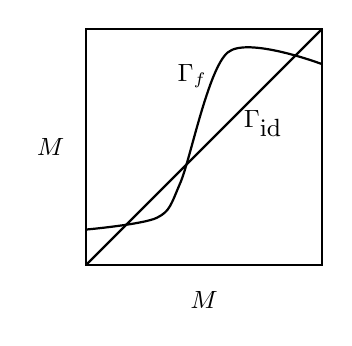
\begin{tikzpicture}[scale=1.5]
    \draw [thick] (0,0) -- (2,0) -- (2,2)--(0,2)--cycle;
        \draw [thick] (0,0)  -- (2,2);
        \draw [thick] plot [smooth] coordinates {(0,.3) (.6,.4) (.8,.7)(1.2,1.8) (2,1.7) };
        \node at (.9,1.6) {\small $\Gamma_f$};
        \node at (1.5,1.2) {\small $\Gamma_{\textrm{id}}$};
        \node at (1,-.3) {\small $M$};
                \node at (-.3,1) {\small $M$};
  \end{tikzpicture}
\end{center}



Let $X$ is a smooth vector field on $M$ and $\varphi_t$ is a flow generated by $X$. Then, the index of a zero point $p$ of $X$ is defined by
$$
\textrm{ind}_p (X) =\textrm{ind}_p(\varphi_t)~.
$$
Since the flow $\varphi_t$ is homotopic to the identity $\varphi_t\simeq \id$, $L(\varphi_t)$ is equal to the Euler characteristic.
$$
    L(\varphi_t) =\sum_{i \geq 0} (-1)^i \Tr(\id:H_i(M;\bR) \to H_i(M;\bR)).=\sum_{i \geq 0} (-1)^i \dim H_i(M;\bR) =\chi(M)
$$
Therefore, we obtain:
\bthm[Poincar\'e-Hopf theorem]
The Euler characteristics is the sum of indices over isolated fixed points
$$
\chi(M)=\sum_{p} \textrm{ind}_p (X)
$$
\ethm


\begin{minipage}[b]{6.5cm}
\includegraphics[width=5.5cm]{pictures/vector-fields}
\end{minipage}
\begin{minipage}[b]{8cm}
\includegraphics[width=8.5cm]{pictures/vector-field-indices}
\end{minipage}


This theorem was introduced in \S\ref{sec:Euler}. There is another important ``fixed point theorem'' due to Brouwer, which we delegate to \cite{milnor1965topology}.























\end{document}
